\documentclass[12pt,a4paper]{article}

% ─── Page Layout ───────────────────────────────────────────────────────────────
\usepackage[a4paper, margin=0.8in, headheight=14pt]{geometry}

% ─── Fonts (XeLaTeX) ───────────────────────────────────────────────────────────
\usepackage{fontspec}
\usepackage{unicode-math}
\setmainfont{TeX Gyre Pagella}
\setmonofont[Scale=0.88]{TeX Gyre Cursor}
\setmathfont{Latin Modern Math}

% ─── Packages ──────────────────────────────────────────────────────────────────
\usepackage{xcolor}
\usepackage{colortbl}
\usepackage{titlesec}
\usepackage{enumitem}
\usepackage{tabularx}
\usepackage{booktabs}
\usepackage{array}
\usepackage{amsmath}
\usepackage{tikz}
\usetikzlibrary{shapes.geometric, arrows.meta, positioning, calc, fit, decorations.pathreplacing, patterns}
\usepackage[american]{circuitikz}
\usepackage{tcolorbox}
\tcbuselibrary{skins, breakable}
\usepackage{hyperref}
\usepackage{fancyhdr}
\usepackage{graphicx}
\usepackage{microtype}
\hyphenpenalty=10000
\exhyphenpenalty=10000
\sloppy
\usepackage{caption}
\usepackage{setspace}
\usepackage{multirow}
\usepackage{tocloft}

% ─── Q&A helper ────────────────────────────────────────────────────────────────
\newcommand{\Q}[1]{\textbf{#1}\par\noindent\ignorespaces}

% ─── Colour Palette ────────────────────────────────────────────────────────────
\definecolor{myred}{RGB}{196,30,58}
\definecolor{mydark}{RGB}{30,30,50}
\definecolor{mygreen}{RGB}{14,120,80}
\definecolor{myteal}{RGB}{0,130,140}
\definecolor{myamber}{RGB}{180,100,0}
\definecolor{mypurple}{RGB}{100,30,160}
\definecolor{mygray}{RGB}{246,247,249}
\definecolor{mgframe}{RGB}{180,185,200}
\definecolor{watermark}{RGB}{145,150,170}
\definecolor{hdrred}{RGB}{250,232,235}
\definecolor{hdrgreen}{RGB}{220,244,233}
\definecolor{hdrteal}{RGB}{220,242,244}
\definecolor{hdramber}{RGB}{253,242,215}
\definecolor{hdrpurple}{RGB}{238,228,255}
\definecolor{hdrgray}{RGB}{238,240,245}
\definecolor{rowalt}{RGB}{250,251,253}

% ─── Section Formatting ────────────────────────────────────────────────────────
\titleformat{\section}{\large\bfseries\color{myred}}{\thesection.}{0.5em}{}[\vspace{1pt}{\color{myred}\rule{\linewidth}{0.8pt}}]
\titleformat{\subsection}{\normalsize\bfseries\color{myteal}}{\thesubsection}{0.5em}{}
\titlespacing*{\section}{0pt}{18pt}{7pt}
\titlespacing*{\subsection}{0pt}{11pt}{4pt}

% ─── Paragraph ─────────────────────────────────────────────────────────────────
\setlength{\parindent}{0pt}
\setlength{\parskip}{4pt}

% ─── TOC Styling ───────────────────────────────────────────────────────────────
\renewcommand{\cfttoctitlefont}{\large\bfseries\color{myred}}
\renewcommand{\cftaftertoctitle}{\par\noindent{\color{myred}\rule{\linewidth}{0.8pt}}}
\setlength{\cftbeforetoctitleskip}{0pt}
\setlength{\cftaftertoctitleskip}{6pt}
\renewcommand{\cftsecfont}{\normalsize\bfseries\color{mydark}}
\renewcommand{\cftsecpagefont}{\normalsize\bfseries\color{mydark}}
\renewcommand{\cftsecleader}{\cftdotfill{\cftdotsep}}
\setlength{\cftbeforesecskip}{7pt}
\renewcommand{\cftsubsecfont}{\small\color{mydark}}
\renewcommand{\cftsubsecpagefont}{\small\color{mydark}}
\setlength{\cftbeforesubsecskip}{3pt}
\setlength{\cftsubsecindent}{1.4em}

% ─── Table helpers ─────────────────────────────────────────────────────────────
\renewcommand{\arraystretch}{1.45}
\setlength{\tabcolsep}{6pt}
\arrayrulecolor{mydark}
\newcolumntype{B}[1]{>{\small\bfseries\raggedright\arraybackslash}m{#1}}
\newcolumntype{Y}{>{\small\raggedright\arraybackslash}X}
\renewcommand{\tabularxcolumn}[1]{m{#1}}

% ─── Header / Footer ───────────────────────────────────────────────────────────
\pagestyle{fancy}
\fancyhf{}
\fancyhead[L]{\small\color{myred}\textbf{PE-EC802C}\;\color{mydark}--- VLSI Design Automation}
\fancyhead[R]{\small\color{myteal}\textbf{Module 3 Notes}}
\fancyfoot[C]{\small\color{mydark}\thepage}
\fancyfoot[R]{\small\color{watermark}\textit{\copyright\ Biraj Sarkar}}
\renewcommand{\headrulewidth}{0.5pt}
\renewcommand{\footrulewidth}{0.3pt}

% ─── Hyperref ──────────────────────────────────────────────────────────────────
\hypersetup{colorlinks=true, linkcolor=myteal, urlcolor=myteal,
  pdfauthor={Biraj Sarkar}, pdftitle={PE-EC802C --- Module 3 Notes}}

% ─── tcolorbox styles ──────────────────────────────────────────────────────────
\tcbset{
  tikzbox/.style={colback=mygray, colframe=mgframe, boxrule=0.6pt, arc=4pt,
    left=8pt, right=8pt, top=6pt, bottom=6pt,
    colbacktitle=mgframe, coltitle=mydark, fonttitle=\small\bfseries},
  defbox/.style={colback=hdrgreen, colframe=mygreen, boxrule=0.8pt, arc=4pt,
    left=9pt, right=9pt, top=6pt, bottom=6pt,
    colbacktitle=mygreen, coltitle=white, fonttitle=\small\bfseries},
  formulabox/.style={colback=hdrteal, colframe=myteal, boxrule=0.8pt, arc=4pt,
    left=9pt, right=9pt, top=7pt, bottom=7pt,
    colbacktitle=myteal, coltitle=white, fonttitle=\small\bfseries},
  examplebox/.style={colback=hdramber, colframe=myamber, boxrule=0.8pt, arc=4pt,
    left=9pt, right=9pt, top=6pt, bottom=6pt,
    colbacktitle=myamber, coltitle=white, fonttitle=\small\bfseries},
  masonbox/.style={colback=hdrpurple, colframe=mypurple, boxrule=0.8pt, arc=4pt,
    left=9pt, right=9pt, top=6pt, bottom=6pt,
    colbacktitle=mypurple, coltitle=white, fonttitle=\small\bfseries},
  exambox/.style={colback=hdrpurple, colframe=mypurple, boxrule=1pt, arc=5pt,
    left=10pt, right=10pt, top=8pt, bottom=8pt,
    colbacktitle=mypurple, coltitle=white, fonttitle=\bfseries,
    breakable, title after break={\textbf{Frequently Asked / Viva Questions (contd.)}}}
}
\tcbset{breakable}

% ─── TikZ styles ───────────────────────────────────────────────────────────────
\tikzset{
  block/.style={rectangle, draw=myteal, fill=hdrteal,
    text width=2.4cm, align=center, minimum height=0.95cm,
    font=\small, rounded corners=3pt, line width=0.7pt},
  redblock/.style={rectangle, draw=myred, fill=hdrred,
    text width=2.4cm, align=center, minimum height=0.95cm,
    font=\small, rounded corners=3pt, line width=0.7pt},
  sumjunc/.style={circle, draw=myamber, fill=hdramber,
    minimum size=0.62cm, font=\small, line width=0.8pt},
  arrow/.style={-Stealth, thick, color=mydark},
  line/.style={thick, color=mydark}
}

% ═══════════════════════════════════════════════════════════════════════════════
\begin{document}
% ═══════════════════════════════════════════════════════════════════════════════

\begin{center}
  {\LARGE\bfseries\color{myred} PE-EC802C --- VLSI Design Automation}\\[5pt]
  {\normalsize\color{mydark} Semester VIII \quad$\bullet$\quad 3L:0T:0P \quad$\bullet$\quad 3 Credits}\\[3pt]
  {\normalsize\color{myteal}\textbf{Module 3: Floorplanning \& Routing}}\\[3pt]
  {\small\color{mydark} CGEC \;$|$\; B.Tech ECE (2023--27) \;$|$\; \textit{Biraj Sarkar}}
\end{center}
\vspace{2pt}
\noindent{\color{myred}\rule{\linewidth}{1.5pt}}
\vspace{2pt}

\hypersetup{linkcolor=mydark}
\tableofcontents
\hypersetup{linkcolor=myteal}
\newpage

% ===============================================================================
\section{Circuit Floorplanning}
% ===============================================================================

\begin{tcolorbox}[defbox, title={Circuit Floorplanning}]
  \textbf{Floorplanning} is the process of identifying the physical shapes, aspect ratios, and positions of the major functional blocks (macros) on the silicon die. It optimizes the chip area and estimates the total wirelength prior to the cell placement phase.
\end{tcolorbox}

\subsection{Slicing vs. Non-Slicing Floorplans}
\begin{itemize}[leftmargin=*, itemsep=2pt]
  \item \textbf{Slicing Floorplan:} A floorplan that can be obtained by recursively partitioning a rectangle into two smaller rectangles using either a horizontal or vertical cut line.
  \item \textbf{Non-Slicing Floorplan:} A floorplan that cannot be partitioned using recursive bisection lines (contains cyclical structures like a wheel configuration).
\end{itemize}

\subsection{Polish Expressions and Slicing Trees}
Slicing floorplans are represented using two equivalent models:
\begin{itemize}[leftmargin=*, itemsep=2pt]
  \item \textbf{Slicing Tree:} A binary tree where the leaf nodes represent the blocks ($A, B, C, \dots$) and the internal nodes represent the cuts ($+$ for horizontal, $*$ for vertical).
  \item \textbf{Polish Expression:} A postfix representation of the slicing tree. A Polish expression is \textit{normalized} if it contains no consecutive identical operators (e.g., $AB++$ is normalized to $AB+C+$).
\end{itemize}

\begin{tcolorbox}[tikzbox, title={Slicing Floorplan, Tree, and Polish Expression}]
\centering
\begin{minipage}{0.31\linewidth}
\centering
\textbf{Floorplan Layout:}\par\noindent
\vspace{6pt}
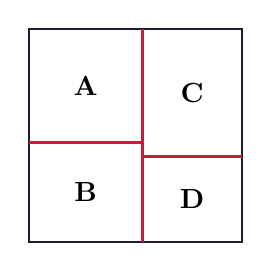
\begin{tikzpicture}[scale=0.9]
  % Outer boundary
  \draw[draw=mydark, thick] (0,0) rectangle (3.0,3.0);
  % Vertical slice at x=1.6
  \draw[line, color=myred, line width=1pt] (1.6,0) -- (1.6,3.0);
  % Horizontal slice in left section at y=1.4
  \draw[line, color=myred, line width=1pt] (0,1.4) -- (1.6,1.4);
  % Horizontal slice in right section at y=1.2
  \draw[line, color=myred, line width=1pt] (1.6,1.2) -- (3.0,1.2);
  
  % Labels
  \node at (0.8,2.2) {\textbf{A}};
  \node at (0.8,0.7) {\textbf{B}};
  \node at (2.3,2.1) {\textbf{C}};
  \node at (2.3,0.6) {\textbf{D}};
\end{tikzpicture}
\end{minipage}\hfill
\begin{minipage}{0.35\linewidth}
\centering
\textbf{Slicing Tree:}\par\noindent
\vspace{6pt}
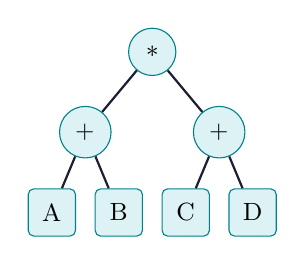
\begin{tikzpicture}[scale=0.85, every node/.style={circle, draw=myteal, fill=hdrteal, minimum size=0.6cm, font=\small}]
  \node (root) at (1.5,2.4) {$*$};
  \node (L) at (0.5,1.2) {$+$};
  \node (R) at (2.5,1.2) {$+$};
  \node[rectangle, rounded corners=2pt] (A) at (0,0) {A};
  \node[rectangle, rounded corners=2pt] (B) at (1.0,0) {B};
  \node[rectangle, rounded corners=2pt] (C) at (2.0,0) {C};
  \node[rectangle, rounded corners=2pt] (D) at (3.0,0) {D};

  \draw[line] (root) -- (L);
  \draw[line] (root) -- (R);
  \draw[line] (L) -- (A);
  \draw[line] (L) -- (B);
  \draw[line] (R) -- (C);
  \draw[line] (R) -- (D);
\end{tikzpicture}
\end{minipage}\hfill
\begin{minipage}{0.31\linewidth}
\centering
\textbf{Polish Expression:}\par\noindent
\vspace{25pt}
{\large\bfseries\color{mypurple} AB+CD+*}
\vspace{15pt}
\begin{itemize}[leftmargin=*, label=$\bullet$]
  \item \textbf{Left Sub:} $AB+$
  \item \textbf{Right Sub:} $CD+$
  \item \textbf{Merged by:} $*$
\end{itemize}
\end{minipage}
\end{tcolorbox}

\subsection{Shape Functions and Sizing Optimization}
The shape function of a block describes its width $w$ as a function of height $h$.
\begin{itemize}[leftmargin=*, itemsep=2pt]
  \item \textbf{For a Horizontal Cut ($+$) of blocks 1 and 2:}
        \begin{equation}
          w = \max(w_1, w_2), \quad h = h_1 + h_2
        \end{equation}
  \item \textbf{For a Vertical Cut ($*$) of blocks 1 and 2:}
        \begin{equation}
          w = w_1 + w_2, \quad h = \max(h_1, h_2)
        \end{equation}
\end{itemize}
Sizing algorithms recursively combine child shape functions at internal tree nodes using horizontal or vertical addition rules, choosing the combination that minimizes total layout area.

% ===============================================================================
\section{Circuit Routing}
% ===============================================================================

Routing is divided into two sequential steps to manage complexity:
\begin{enumerate}[leftmargin=*, itemsep=2pt]
  \item \textbf{Global Routing:} Divides the chip into a grid of routing channels, planning a coarse pathway for each net through grid regions without assigning specific wire tracks.
  \item \textbf{Detailed Routing:} Assigns nets to precise metal tracks and layers within the channels planned by the global router.
\end{enumerate}

\subsection{Classification of Routing Problems \& Methods}
Routing problems are classified based on the geometrical constraints and abstraction levels:
\begin{itemize}[leftmargin=*, itemsep=3pt]
  \item \textbf{Local Routing Problems:} Connecting terminal pins within a localized region.
        \begin{itemize}[leftmargin=*, label=$\bullet$, itemsep=1pt]
          \item \textbf{Grid-based Routing:} The routing area is discretized into a uniform grid. Wires can only run along grid tracks, and vias can only be placed at grid intersections. Easy to model but consumes significant memory.
          \item \textbf{Gridless (Continuous) Routing:} Wires can be placed at any coordinate, restricted only by design rule boundaries (minimum spacing and width). Highly memory efficient and supports variable wire widths.
        \end{itemize}
  \item \textbf{Area Routing:} Connecting pins across a general 2D area (often containing arbitrary blockages and obstacles). Examples include maze routers (Lee's, Soukup's) and line-probe routers (Mikami-Tabuchi, Hightower).
  \item \textbf{Channel Routing:} Connecting pins along two parallel rows (boundaries) using horizontal segments on one layer and vertical segments on another (detailed in Section 4).
\end{itemize}

\subsection{Global Routing \& Algorithms}
Global routing plans the approximate path of each net to avoid congestion across the chip area. The chip is modeled as a \textbf{Grid Graph} $G_c = (V_c, E_c)$, where each vertex $v_i$ represents a routing region (bin) and each edge $e_{ij}$ represents the boundary between adjacent regions with a capacity constraint $c_{ij}$ (maximum number of wires allowed to cross).

\subsubsection{Key Global Routing Algorithms}
\begin{enumerate}[leftmargin=*, itemsep=4pt]
  \item \textbf{Rectilinear Minimum Steiner Tree (RMST):} A Steiner tree connects a set of pins by introducing auxiliary vertices called \textbf{Steiner points} to minimize total wirelength using only horizontal and vertical segments. Finding the RMST is NP-complete, so heuristics (e.g., Hwang's theorem, FLUTE) are used.
  \item \textbf{Rectilinear Steiner Arborescence (RSA):} A directed Steiner tree routed from a source pin (root) to multiple sink pins such that the path from the root to any sink is a shortest rectilinear path.
  \item \textbf{Sequential Routing with Rip-up and Re-route:}
        \begin{itemize}[leftmargin=*, label=$\bullet$, itemsep=1pt]
          \item Router routes nets one by one sequentially (e.g. using Dijkstra's algorithm).
          \item Early nets take the shortest paths, causing congestion and capacity violations for later nets.
          \item \textbf{Rip-up and Re-route:} Congested nets are ripped up, edge weights are increased to penalize congestion, and the nets are rerouted until all capacity constraints are satisfied.
        \end{itemize}
  \item \textbf{ILP-based Global Routing:} Formulates global routing as a multi-commodity flow problem to route all nets simultaneously, optimizing total wirelength subject to capacity constraints.
\end{enumerate}

\subsection{Lee's Maze Routing Algorithm}
Lee's algorithm uses a Breadth-First Search (BFS) grid expansion technique to find the shortest path between a source ($S$) and target ($T$) grid cell. It guarantees finding a path if one exists and always finds the shortest path.

\subsubsection{Algorithmic Flow}
\begin{enumerate}[leftmargin=*, itemsep=2pt]
  \item \textbf{Initialization:} Label the source cell $S$ with $0$. Set wave counter $i = 0$.
  \item \textbf{Wave Expansion:} Find all unlabeled neighbor cells of cells labeled $i$. If a neighbor is target $T$, stop. Otherwise, label them $i+1$. Repeat this expansion until the target is reached or no more cells can be labeled (blocked).
  \item \textbf{Traceback:} From $T$, trace back to $S$ by moving to neighbor cells with decreasing labels ($i, i-1, \dots, 0$).
  \item \textbf{Clear:} Clear all numbers on the grid.
\end{enumerate}

\begin{tcolorbox}[tikzbox, title={Lee's Maze Router BFS Grid Expansion}]
\centering
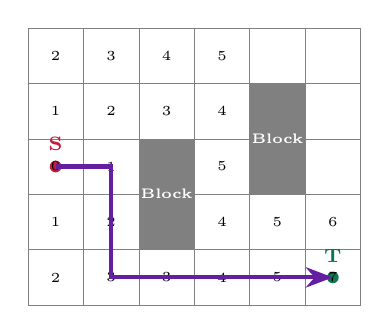
\begin{tikzpicture}[scale=0.88]
  % Draw Grid
  \draw[step=0.8cm, gray, very thin] (0,0) grid (4.8,4.0);
  
  % Obstacles
  \fill[gray] (1.6,0.8) rectangle (2.4,2.4);
  \node[color=white, font=\tiny\bfseries] at (2.0,1.6) {Block};
  \fill[gray] (3.2,1.6) rectangle (4.0,3.2);
  \node[color=white, font=\tiny\bfseries] at (3.6,2.4) {Block};

  % Source & Target
  \node[circle, fill=myred, inner sep=1.5pt] (S) at (0.4,2.0) {};
  \node[above=2pt, font=\scriptsize\bfseries\color{myred}] at (0.4,2.0) {S};
  
  \node[circle, fill=mygreen, inner sep=1.5pt] (T) at (4.4,0.4) {};
  \node[above=2pt, font=\scriptsize\bfseries\color{mygreen}] at (4.4,0.4) {T};

  % Wave numbers
  \node[font=\tiny] at (0.4,2.0) {0};
  \node[font=\tiny] at (0.4,2.8) {1};
  \node[font=\tiny] at (0.4,1.2) {1};
  \node[font=\tiny] at (1.2,2.0) {1};

  \node[font=\tiny] at (0.4,3.6) {2};
  \node[font=\tiny] at (1.2,2.8) {2};
  \node[font=\tiny] at (1.2,1.2) {2};
  \node[font=\tiny] at (0.4,0.4) {2};

  \node[font=\tiny] at (1.2,3.6) {3};
  \node[font=\tiny] at (2.0,2.8) {3};
  \node[font=\tiny] at (2.0,0.4) {3};
  \node[font=\tiny] at (1.2,0.4) {3};

  \node[font=\tiny] at (2.0,3.6) {4};
  \node[font=\tiny] at (2.8,2.8) {4};
  \node[font=\tiny] at (2.8,1.2) {4};
  \node[font=\tiny] at (2.8,0.4) {4};

  \node[font=\tiny] at (2.8,3.6) {5};
  \node[font=\tiny] at (2.8,2.0) {5};
  \node[font=\tiny] at (3.6,1.2) {5};
  \node[font=\tiny] at (3.6,0.4) {5};

  \node[font=\tiny] at (4.4,1.2) {6};
  \node[font=\tiny] at (4.4,0.4) {7};

  % Traceback Path
  \draw[arrow, color=mypurple, line width=1.5pt] (0.4,2.0) -- (1.2,2.0) -- (1.2,1.2) -- (1.2,0.4) -- (2.0,0.4) -- (2.8,0.4) -- (3.6,0.4) -- (4.4,0.4);
\end{tikzpicture}
\tcblower
Shortest path found: $S(0) \rightarrow (1) \rightarrow (2) \rightarrow (3) \rightarrow (4) \rightarrow (5) \rightarrow (6) \rightarrow T(7)$. Grid obstacles force the router to loop around the bottom.
\end{tcolorbox}

\subsubsection{Limitations of Lee's Router}
\begin{itemize}[leftmargin=*, itemsep=2pt]
  \item \textbf{High Memory Overhead:} Storing wave expansion numbers on a large grid of size $N \times N$ requires $O(N^2)$ memory.
  \item \textbf{Slow Execution:} Expanding wavefronts in all directions behaves like a BFS, taking $O(N^2)$ time.
  \item \textbf{Optimizations:} \textbf{Soukup's Router} uses a heuristic search (DFS) towards the target to speed up propagation, falling back to Lee's algorithm only when blocked. \textbf{Line-Probe Router} routes lines instead of cells, reducing memory usage.
\end{itemize}

% ===============================================================================
\section{Channel Routing}
% ===============================================================================

\begin{tcolorbox}[defbox, title={Channel Routing}]
  \textbf{Channel Routing} is a detailed routing technique that connects terminal pins along two parallel rows (top and bottom boundaries of a horizontal channel) using horizontal wire segments on one metal layer and vertical wire segments on a different metal layer.
\end{tcolorbox}

\subsection{Left-Edge Algorithm}
The Left-Edge algorithm is a greedy track allocation algorithm that routes nets in a single pass from left to right.
\begin{enumerate}[leftmargin=*, itemsep=2pt]
  \item Sort all nets in ascending order of their left-most pin $x$-coordinate.
  \item Select the first unrouted net and assign it to the first available track.
  \item Scan left to right to find the next unrouted net whose left boundary does not overlap with the previously routed net on the same track. Assign it to the same track.
  \item Repeat step 3 until no more nets can fit in the current track.
  \item Open a new track and repeat steps 2-4 until all nets are routed.
\end{enumerate}

\subsection{Horizontal and Vertical Constraint Graphs}
To prevent wire overlaps, the channel router must respect two types of constraints:
\begin{itemize}[leftmargin=*, itemsep=2pt]
  \item \textbf{Horizontal Constraints:} Nets overlapping in their horizontal span cannot share the same track. (Modeled using interval graphs).
  \item \textbf{Vertical Constraints:} If net $A$'s top pin is directly above net $B$'s bottom pin at some column, net $A$'s horizontal wire segment must be placed in a track above net $B$'s track to avoid vertical wire overlaps. (Represented as a directed \textbf{Vertical Constraint Graph (VCG)} where edge $A \rightarrow B$ means track($A$) $>$ track($B$)).
\end{itemize}

\newpage

% ═══════════════════════════════════════════════════════════════════════════════
% QUICK REVISION PAGE
% ═══════════════════════════════════════════════════════════════════════════════
\begin{center}
  {\large\bfseries\color{myred} Quick Revision — Module 3}\\[3pt]
  {\small\color{mydark} Floorplanning \& Routing $|$ PE-EC802C}
\end{center}
\noindent{\color{myred}\rule{\linewidth}{1.2pt}}
\vspace{8pt}

\begin{tcolorbox}[formulabox, title={\textbf{Key Formulas and Metrics at a Glance}}]
\renewcommand{\arraystretch}{1.35}
\begin{tabularx}{\linewidth}{B{5.0cm} X}
  Horizontal Cut (+) & $h_{\text{parent}} = h_1 + h_2, \quad w_{\text{parent}} = \max(w_1, w_2)$ \\[4pt]
  Vertical Cut (*) & $w_{\text{parent}} = w_1 + w_2, \quad h_{\text{parent}} = \max(h_1, h_2)$ \\[4pt]
  Lee's Wave Expansion & $\text{Label value } L \le |x_s - x_t| + |y_s - y_t| \quad (\text{Manhattan limit})$ \\[4pt]
  Channel Routing Tracks & $\text{Lower Bound on Tracks } = \max_x d(x) \quad (d_{\max} \text{ density})$
\end{tabularx}
\tcblower
The maximum channel density $d_{\max}$ represents the minimum number of tracks required to route the channel without overlap.
\end{tcolorbox}

\vspace{6pt}

\begin{tcolorbox}[defbox, title={\textbf{One-Line Definitions}}]
\begin{itemize}[leftmargin=*, itemsep=3pt, topsep=0pt]
  \item \textbf{Floorplanning:} Finding optimal block locations and aspect ratios prior to cell placement.
  \item \textbf{Slicing Cut:} A cut line that splits a floorplan region completely into two sub-regions.
  \item \textbf{Polish Expression:} A postfix notation string describing slicing sequences and leaf blocks.
  \item \textbf{Shape Function:} A curve or step function representing possible width and height values of a block.
  \item \textbf{Maze Routing:} Routing algorithms that find grid-based paths between pins around layout obstacles.
  \item \textbf{Traceback:} The path reconstruction phase of Lee's algorithm working backward from target to source.
  \item \textbf{Left-Edge Algorithm:} A track allocation algorithm that routes nets sorted by their left-most coordinate.
  \item \textbf{Vertical Constraint Graph:} A directed graph indicating which net must be placed above another to avoid overlaps.
\end{itemize}
\end{tcolorbox}

\vspace{6pt}

\begin{tcolorbox}[exambox, title={\textbf{Frequently Asked / Viva Questions}}]
\begin{enumerate}[leftmargin=*, topsep=0pt, label=\textbf{Q\arabic*.}, itemsep=6pt]
  \item \Q{What is a normalized Polish expression, and why is it important?}
        A Polish expression is normalized if it has no consecutive identical operators (e.g. $AB++$ is not normalized, whereas $AB+C+$ is). Normalization guarantees a 1-to-1 mapping between Polish expressions and slicing floorplans, which reduces the search space during optimization.
        
  \item \Q{Why is floorplanning done before placement?}
        Floorplanning handles large blocks (macros) and defines the global silicon structure. Placing small standard cells directly without placing macros first would lead to congestion, wiring bottlenecks, and poor cell distribution.
        
  \item \Q{Explain the wave expansion step in Lee's maze routing algorithm.}
        Starting at the source node, neighbors are labeled with 1. Then, all unlabeled neighbors of 1 are labeled with 2. This process is repeated, labeling neighbors of $i$ with $i+1$, until the target cell is reached. This BFS propagation guarantees finding the shortest path.
        
  \item \Q{What are the main drawbacks of Lee's maze router?}
        (1) It uses $O(N^2)$ memory to store the grid cell states and label numbers. (2) It is slow ($O(N^2)$ time) because the wavefront expands in all directions, looking like a growing circle, which explores many unnecessary grid nodes.
        
  \item \Q{How does Soukup's router improve on Lee's algorithm?}
        Soukup's router uses a depth-first search (DFS) strategy to route directly toward the target cell. If it hits an obstacle, it switches to Lee's BFS expansion to find a way around the obstacle, then switches back to DFS. This reduces the search time significantly.
        
  \item \Q{Explain the vertical constraint in channel routing with an example.}
        If Net 1 has a pin on the top row of a channel at column 3, and Net 2 has a pin on the bottom row at column 3, the vertical wire segments of Net 1 and Net 2 both lie along column 3. To prevent a short circuit, Net 1's horizontal wire segment must be placed in a track above Net 2's track.
        
  \item \Q{What is a dogleg in channel routing, and why is it used?}
        A dogleg is a vertical wire segment that splits a net's horizontal wire segment across different tracks. It is used to resolve cyclical conflicts in Vertical Constraint Graphs, reducing the total number of tracks needed to route the channel.
        
  \item \Q{How does the Left-Edge algorithm route nets?}
        It first sorts all nets by their left-most pin coordinates. It then processes nets in order, placing as many non-overlapping nets as possible into the first track. When no more nets can fit, it moves to the next track and repeats the process until all nets are routed.
        
  \item \Q{What is the difference between slicing and non-slicing floorplans?}
        A slicing floorplan can be completely partitioned into individual blocks using recursive vertical and horizontal cuts. A non-slicing floorplan cannot be divided this way because it contains wheel-like cycles of blocks.
        
  \item \Q{What is channel density, and why is it important?}
        Channel density is the maximum number of nets crossing any vertical slice of a routing channel. It represents the mathematical lower bound on the number of tracks required to route the channel without overlaps.
\end{enumerate}
\end{tcolorbox}

\vspace{6pt}

\begin{tcolorbox}[tikzbox, title={\textbf{Comparison Snapshot}}]
\textbf{Slicing vs. Non-Slicing Floorplans:}\par\vspace{6pt}\noindent
{\renewcommand{\arraystretch}{1.35}%
\begin{tabularx}{\linewidth}{|B{3.2cm}|Y|Y|}
\hline
\textbf{Feature} & \textbf{Slicing Floorplan} & \textbf{Non-Slicing Floorplan} \\
\hline
Representation & Binary trees, Polish expressions. & Constraint graphs (BSG, Sequence Pairs). \\
\hline
Complexity & Optimization is fast ($O(n \log n)$). & Optimization is slow and computationally complex. \\
\hline
Optimal Sizing & Can be solved optimally in polynomial time. & Sizing is NP-complete. \\
\hline
\end{tabularx}}

\vspace{12pt}
\textbf{Global Routing vs. Detailed Routing:}\par\vspace{6pt}\noindent
{\renewcommand{\arraystretch}{1.35}%
\begin{tabularx}{\linewidth}{|B{3.2cm}|Y|Y|}
\hline
\textbf{Feature} & \textbf{Global Routing} & \textbf{Detailed Routing} \\
\hline
Abstraction & Coarse grid, ignores specific tracks. & Actual grid, routes on precise metal tracks. \\
\hline
Objective & Allocates nets to routing regions to avoid congestion. & Resolves layout design rules, placing vias and wires. \\
\hline
Algorithm & Steiner trees, maze routers, network flows. & Left-Edge algorithm, dogleg routers, grid maze. \\
\hline
\end{tabularx}}
\end{tcolorbox}

\end{document}
